\section{Preprocessing: from video to lexicon entry}
\label{sec:preproc}
Every source, whatever its form (a dictionary video per word, a lesson, a recitation in sign, a dataset of clips or a
file of precomputed keypoints), goes through the same pipeline (Figure~\ref{fig:preproc}), so that all signs end up in
one format and can be joined.

\begin{figure}[ht]
\centering
\resizebox{\textwidth}{!}{%
\begin{tikzpicture}[node distance=5mm and 5mm,
  st/.style={draw=navy, rounded corners=2pt, fill=soft, align=center, font=\footnotesize, minimum height=15mm, text width=30mm,
             inner sep=2pt},
  arr/.style={-{Stealth[length=2mm]}, thick, navy}]
  \node[st] (v) {\textbf{1. Source}\\video, lesson,\\recitation, clips};
  \node[st, right=of v] (k) {\textbf{2. Keypoints}\\MediaPipe Holistic:\\33 body, 2$\times$21 hand,\\468 face landmarks};
  \node[st, right=of k] (s) {\textbf{3. Selection}\\50 joints: 8 upper\\body + 2$\times$21 hand;\\face dropped};
  \node[st, right=of s] (n) {\textbf{4. Normalisation}\\neck origin,\\shoulder-width unit,\\25 fps, gaps filled};
  \node[st, below=9mm of n] (c) {\textbf{5. Segmentation}\\cut the sign: hand-\\visible span, captions,\\timestamps, motion};
  \node[st, left=of c] (q) {\textbf{6. Quality filter}\\reject if the hand is\\missing too often\\or the cut is too short};
  \node[st, left=of q] (m) {\textbf{7. Canonical sign}\\DTW medoid of the\\recordings; one other\\signer as template};
  \node[st, left=of m] (e) {\textbf{8. Lexicon entry}\\gloss, source, licence,\\pose, review status,\\religious flag};
  \draw[arr] (v) -- (k); \draw[arr] (k) -- (s); \draw[arr] (s) -- (n); \draw[arr] (n) -- (c);
  \draw[arr] (c) -- (q); \draw[arr] (q) -- (m); \draw[arr] (m) -- (e);
\end{tikzpicture}}
\caption{Preprocessing pipeline applied to every source. Step 5 differs per source (Table~\ref{tab:funnel}).}
\label{fig:preproc}
\end{figure}

\paragraph{Keypoints and shape.} MediaPipe Holistic \cite{mediapipe,mediapipeholistic} returns, for every video frame,
33 body landmarks, 21 landmarks for each hand and 468 face landmarks, in image coordinates with an estimated depth
(Figure~\ref{fig:mediapipe}). We
keep the 8 upper-body joints needed to place the arms (nose, neck as the mid-point of the shoulders, and both shoulders,
elbows and wrists) and all 42 hand landmarks, which carry the hand shape (Figure~\ref{fig:layout}). Each sign is
therefore a tensor of shape $[T, 50, 3]$: $T$ frames at 25 frames per second, 50 joints, and $(x, y, z)$. The face is
not kept yet; it carries the non-manual grammar of sign languages and is planned (Chapter~\ref{sec:discussion}).

\begin{figure}[ht]
\centering
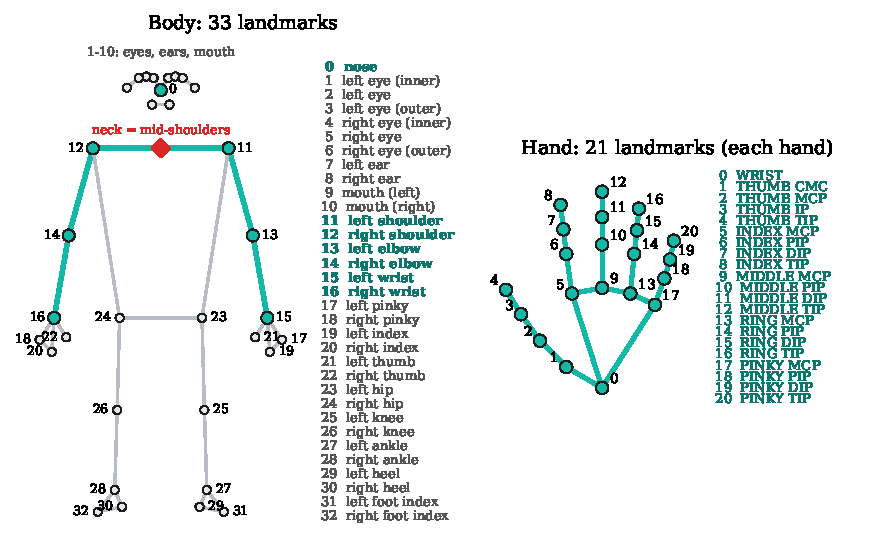
\includegraphics[width=\textwidth]{figures/mediapipe_landmarks.pdf}
\caption{MediaPipe Holistic landmarks, numbered as in its definitions (schematic, subject facing the viewer). Teal and
bold: the body landmarks Isharati keeps (nose, shoulders, elbows, wrists), plus the neck computed as the mid-point of the
shoulders (red); all 21 landmarks of each hand are kept. Grey: discarded (face detail, hand points of the body model,
hips and legs). The 468 face-mesh landmarks are not shown.}
\label{fig:mediapipe}
\end{figure}

\paragraph{Normalisation, Palm Orientation, and Glitch Elimination.}
Raw keypoints extracted across heterogeneous cameras exhibit perspective distortion, coordinate jitter, and catastrophic joint ``glitching'' during rapid wrist rotations or partial finger occlusions. To produce natural, glitch-free animations on 3D avatars and avoid kinematic artifacts, we apply a multi-stage geometric normalization pipeline:
\begin{enumerate}[leftmargin=*,itemsep=2pt]
  \item \textbf{Anthropometric Invariance:} The neck serves as the invariant spatial origin, and the clip's median shoulder width defines the unit scalar (Equation~\ref{eq:norm_pose} in Chapter~\ref{sec:method}). Frames are resampled to 25\,fps, with detection dropouts linearly interpolated.
  \item \textbf{Coordinate System Flipping and Depth Alignment:} Standard computer vision coordinates place $+Y$ downward (screen space) with arbitrary camera $Z$ scaling. We flip the vertical axis ($Y \gets -Y$) and rescale torso depth ($Z_{\text{torso}} \gets 0.5 \times Z_{\text{raw}}$) while preserving full hand dynamic depth ($Z_{\text{hands}} \gets 1.0 \times Z_{\text{raw}}$). This decouples subtle finger configurations from exaggerated torso movement.
  \item \textbf{Orthogonal Palm Frame and Normal Vector Construction:} Rather than driving 3D wrist bones via noisy raw Euler angles (which cause gimbal lock and erratic twisting), we construct an orthonormal local coordinate basis $(\mathbf{u}_{\text{palm}}, \mathbf{v}_{\text{palm}}, \mathbf{w}_{\text{palm}})$ for each hand:
  \begin{equation}
  \mathbf{u} = \frac{\mathbf{p}_{\text{mid\_mcp}} - \mathbf{p}_{\text{wrist}}}{\lVert \mathbf{p}_{\text{mid\_mcp}} - \mathbf{p}_{\text{wrist}} \rVert_2}, \quad
  \mathbf{v} = \frac{\mathbf{p}_{\text{idx\_mcp}} - \mathbf{p}_{\text{pinky\_mcp}}}{\lVert \mathbf{p}_{\text{idx\_mcp}} - \mathbf{p}_{\text{pinky\_mcp}} \rVert_2}, \quad
  \mathbf{n}_{\text{palm}} = \frac{\mathbf{u} \times \mathbf{v}}{\lVert \mathbf{u} \times \mathbf{v} \rVert_2}.
  \end{equation}
  The primary longitudinal vector $\mathbf{u}$ spans from the wrist (joint 0) to the middle knuckle (joint 9), and the transverse vector $\mathbf{v}$ connects the index knuckle (joint 5) to the pinky knuckle (joint 17). Their cross-product $\mathbf{n}_{\text{palm}}$ yields the true normal vector pointing outward from the palm.
  \item \textbf{Quaternion Hemisphere Continuity and Flip Spike Discarding:} Rotational quaternions $q$ and $-q$ represent the same physical orientation in $SO(3)$, but sudden sign flips between consecutive frames cause catastrophic 360$^\circ$ bone twists (avatar arm ``glitching''). We enforce hemisphere continuity by ensuring $\langle q_t, q_{t-1} \rangle \ge 0$; if negative, $q_t \gets -q_t$. Furthermore, if tracking loss produces an instantaneous angular jump exceeding $\Delta \theta > 2.0\,\text{rad}$ ($114.6^\circ$), the anomalous frame is discarded as an artifact spike, and the preceding stable wrist rotation is frozen and smoothed via spherical linear interpolation (SLERP, $\alpha = 0.55$).
  \item \textbf{Anatomical Clearance and Hyper-Extension Clamping:} To prevent hands from glitching backward through the 3D torso or robes, we enforce a dynamic forward clearance boundary ($Z_{\text{wrist}} \ge Z_{\text{shoulder}} + 0.38 \times L_{\text{arm}}$ whenever the hand crosses the chest midline). Individual finger segments are constrained against backward hyper-extension by projecting joint vectors onto the positive half-space defined by the palm normal $\mathbf{n}_{\text{palm}}$, clamping backward deviation to $\le -0.15 \times L_{\text{segment}}$.
  \item \textbf{Collapsed Hand Pinning:} A hand never detected in a frame (e.g., in one-handed signs or letters) is pinned cleanly to its wrist rather than collapsing to the origin, rendering as a natural resting posture rather than a stray limb.
\end{enumerate}
Figure~\ref{fig:norm} illustrates a raw video clip before and after complete normalization: signs captured from a 1080p studio camera and a 480p mobile video converge onto identical, glitch-free kinematic manifolds. Body proportions are equalized across sources at assembly time (Section~\ref{sec:render}).

\begin{figure}[ht]
\centering
\begin{minipage}{0.40\textwidth}\centering
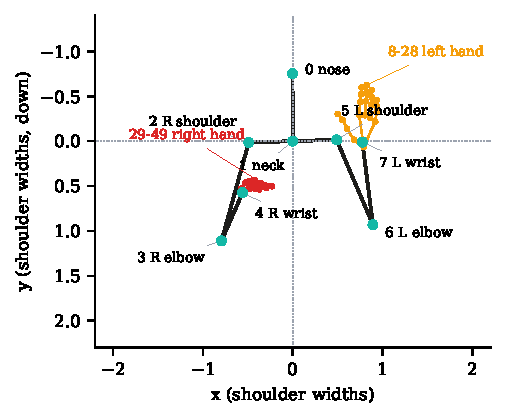
\includegraphics[width=\textwidth]{figures/keypoint_layout.pdf}
\caption{The 50 joints of the Isharati format on a real frame: 8 body joints (teal, numbered), left hand 8--28,
right hand 29--49.}
\label{fig:layout}
\end{minipage}\hfill
\begin{minipage}{0.57\textwidth}\centering
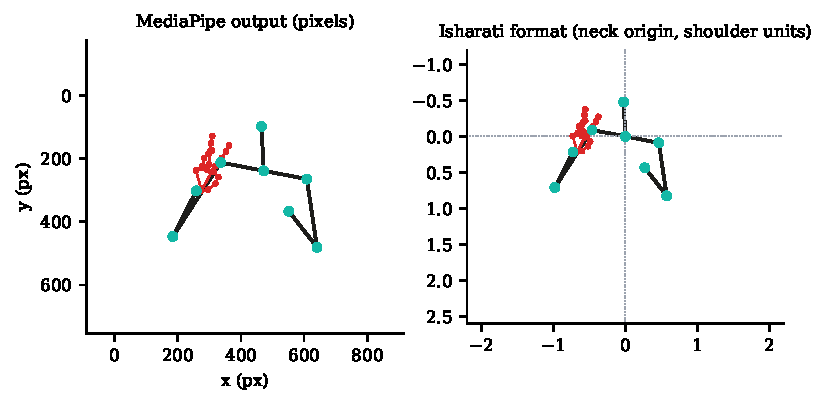
\includegraphics[width=\textwidth]{figures/normalisation.pdf}
\caption{One clip before (MediaPipe pixel coordinates) and after normalisation (neck at the origin, shoulder-width
units).}
\label{fig:norm}
\end{minipage}
\end{figure}

\paragraph{Segmentation and gloss labels.} The gloss of each sign comes from the source: the dataset label, the video
title of a one-word dictionary video, the caption of a lesson, or the word of the religious text being recited. Cutting the sign
out depends on the form of the source:
\begin{itemize}[leftmargin=*,itemsep=1pt]
  \item \textbf{One sign per video} (dictionary channels, WLASL, ASL Citizen, KArSL, T\.{I}D, CISLR, WSLP): the span in
        which a hand is raised and visible; for long clips, the first signing stretch.
  \item \textbf{Captioned lessons} (Tawasol): caption onsets and hand-raised stretches, with the term read per tile
        from contact sheets.
  \item \textbf{Explained dictionaries} (Saudi dictionary): the first motion segment after a coloured label.
  \item \textbf{Qur'an recitation in sign} (Al-Kharj curriculum): the interpreter signs in time with a recitation;
        Whisper word timestamps aligned to the Qur'an text give each word's frames, and the medoid over occurrences of a
        lemma becomes the sign.
  \item \textbf{Continuous narrative and scripture} (Deaf Bible EGCBT): segmented automatically using our continuous
        RoPE Transformer pose segmentation model, followed by monotonic verse-constrained gloss alignment.
  \item \textbf{Islamic term lists} (GDM, Noor): signing stretches anchored by Whisper timestamps of the spoken term.
  \item \textbf{One-word Shorts} (Levantine): the most recurring 0.5--2.5\,s motion segment.
  \item \textbf{Continuous sentence corpora} (ArabSign, Isharah, How2Sign, YouTube-ASL): preserved as continuous utterance sequences for translation and recognition benchmarks, while serving as rich sources for sign mining (e.g., weakly supervised multiple-instance learning on YouTube-ASL and How2Sign to mine individual signs for lexicon gaps, or continuous boundary modeling with our RoPE Transformer), rather than raw unsegmented dictionary entries.
\end{itemize}

\subsection{Continuous Stream Processing with RoPE Transformer Segmentation}
Continuous sign language poses lack discrete audio boundaries when recordings are deaf-first or silent (such as the Deaf Bible EGCBT recordings, where audio tracks register below $-91\,\text{dB}$). In accordance with the system methodology defined in Section~\ref{sec:rope_segmentation}, we apply our pre-trained Rotary Position Embedding (RoPE) Transformer segmentation model~\cite{signsegmentation}\footnote{Sign language pose segmentation repository: \url{https://github.com/sign-language-processing/segmentation}} to partition continuous pose streams into discrete word-level signs without speech alignment.

As formulated in Equation~\eqref{eq:velocity} and Equation~\eqref{eq:rope}, the model operates directly on normalized 3D joint positions and inter-frame velocities ($50 \times 6 = 300$ dimensions), utilizing 4 Transformer encoder layers with RoPE self-attention to label every frame UNK, O, B or I, at about 290 frames per second on a desktop CPU (Section~\ref{sec:results_segmentation}) using the pre-trained \code{model.safetensors} weights (11.5\,MB)\footnote{Pre-trained RoPE Transformer model checkpoint release: \url{https://github.com/sign-language-processing/segmentation/releases/tag/v0.1.0}}. A sign opens at \texttt{B}, continues through \texttt{I}, and closes at \texttt{O} or \texttt{UNK}; spans shorter than 4 frames are rejected. Our benchmark (Section~\ref{sec:results_segmentation}) shows that these boundaries are not yet reliable, in particular when the pose is normalised as in our wrapper rather than as in the package.

\paragraph{Verse-Constrained Monotonic Gloss Alignment.}
Once continuous pose sequences are segmented into millisecond-accurate physical sign boundaries, we align individual gesture segments to Arabic lexical glosses using verse-constrained monotonic dynamic matching. For narrative corpora with parallel text (such as Deaf Bible EGCBT with 47 canonical Scripture stories)\footnote{Deaf Bible Society Egyptian Sign Language chronological catalog: \url{https://deafbible.com/EGCBT}}, the text of each chapter is tokenized into Arabic lemmas. Because sign order in Egyptian Sign Language (ESL) predominantly mirrors chronological narrative order with topic-comment shifts, segment boundaries are mapped monotonically to the ordered set of content words $\{w_1, w_2, \dots, w_K\}$, matching physical duration against lexical syllabic weight. Signs identified with high confidence provide anchor points, establishing ground-truth aligned continuous sign datasets.

\paragraph{Quality filter and canonical sign.} A recording is rejected when the dominant hand is missing in too many
frames (more than 30\% for ASL Citizen, 45\% for the dictionary channels) or the cut is shorter than six frames. Where
several recordings of a gloss exist, the DTW medoid becomes the canonical sign, and a recording by a different signer is
kept as a back-translation template. The entry records the gloss, its aliases, the source, the pose, whether it is a
religious term or a letter, and its review status. Table~\ref{tab:funnel} follows each source from raw material to
the merged lexicons; the merge keeps one sign per gloss, preferring Islamic sources and Deaf-signer dictionaries.

\begin{table}[ht]
\centering\small
\caption{From raw material to lexicon: what each source provided, what was extracted, and how many glosses it
contributes to the merged lexicons (after duplicates are resolved in favour of earlier sources).}
\label{tab:funnel}
\begin{tabularx}{\textwidth}{L{3.6cm} Y r r}
\toprule
Source & Raw material $\rightarrow$ extraction & Signs extracted & Glosses in lexicon \\
\midrule
\multicolumn{4}{l}{\emph{ASL (English mode)}} \\
GDM Islamic signs & 1 video, 40 terms, Whisper-anchored & 41 & 75 \\
Noor For Sign & 1 Ramadan lesson & 7 & 14 \\
Obscure ASL & one-word videos & 102 & 96 \\
ASL Citizen & 83,399 clips of 2,731 glosses; medoid of 3 signers, + 2,259 templates & 2,626 & 2,204 \\
WLASL & 679 glosses not yet covered, up to 2 clips each & 1,241 & 666 \\
\midrule
\multicolumn{4}{l}{\emph{ArSL (Arabic mode)}} \\
KArSL-502 & 4,016 clips, 502 signs, 3 signers; medoid & 502 & 512 \\
Qur'an curriculum & 22 surahs signed with recitation; Whisper--Qur'an alignment & 353 & 332 \\
Tawasol & 154 lesson videos; caption-based cuts & 336 & 205 \\
Saudi / Arabic dictionary explained & 17 videos; label-triggered cuts & 105 & 84 \\
Dictionary channels (unified, Kuwaiti, children's, scouts') & 6,698 one-word clips; 2,137 rejected by the filter & 4,559 & 2,694 \\
Levantine Shorts & 133 videos; recurring-motion cut & 131 & 152 \\
\midrule
\multicolumn{4}{l}{\emph{T\.{I}D (Turkish mode) and ISL (Urdu mode)}} \\
T\.{I}D S\"ozl\"u\u{g}\"u & 5,017 one-word clips (extraction in progress) & 1,308 & 1,374 \\
CISLR & 4,765 words, one reference clip each & 3,965 & 3,965 \\
WSLP 2025 & word-recognition training set & 4,056 & 4,020 \\
\midrule
\multicolumn{4}{l}{\emph{Sentence data (not cut into lexicon signs)}} \\
ArabSign & 6 signers $\times$ 50 sentences, $\sim$30 repetitions & 9,259 sentence poses & -- \\
YouTube-ASL & 391,494 captioned clips (10 parts) & 39,052 (part 1) & -- \\
\bottomrule
\end{tabularx}
\end{table}

\section{The YouTube-ASL keypoint dataset}
\label{sec:ytasl}
YouTube-ASL \cite{youtubeasl} pairs 391,494 sentence clips from 9,422 YouTube videos with their English captions; its
keypoint release \cite{youtubeaslkp} provides, for every clip, MediaPipe landmarks per frame (33 body, 21 per hand, 478
face, in pixels) as one JSON file, 374\,GB in ten archives. We convert it to the Isharati format in the cloud, one
archive at a time so that no local disk is needed: body and hand joints are selected, the face is dropped, coordinates
are normalised, and each archive becomes one compressed array file of clips (about 40$\times$ smaller: 37.5\,GB to
0.91\,GB for the first part) plus a manifest. The manifest has one row per clip: clip and video identifiers, start and
end frame in the source video, number of frames, frame size, the share of frames in which each hand is detected, and the
archive part; the English sentence and the train/dev split are joined from the captions. The result is published as a
Hugging Face dataset with the CC BY 4.0 attribution of the source (Figure~\ref{fig:hf}).

\begin{figure}[ht]
\centering
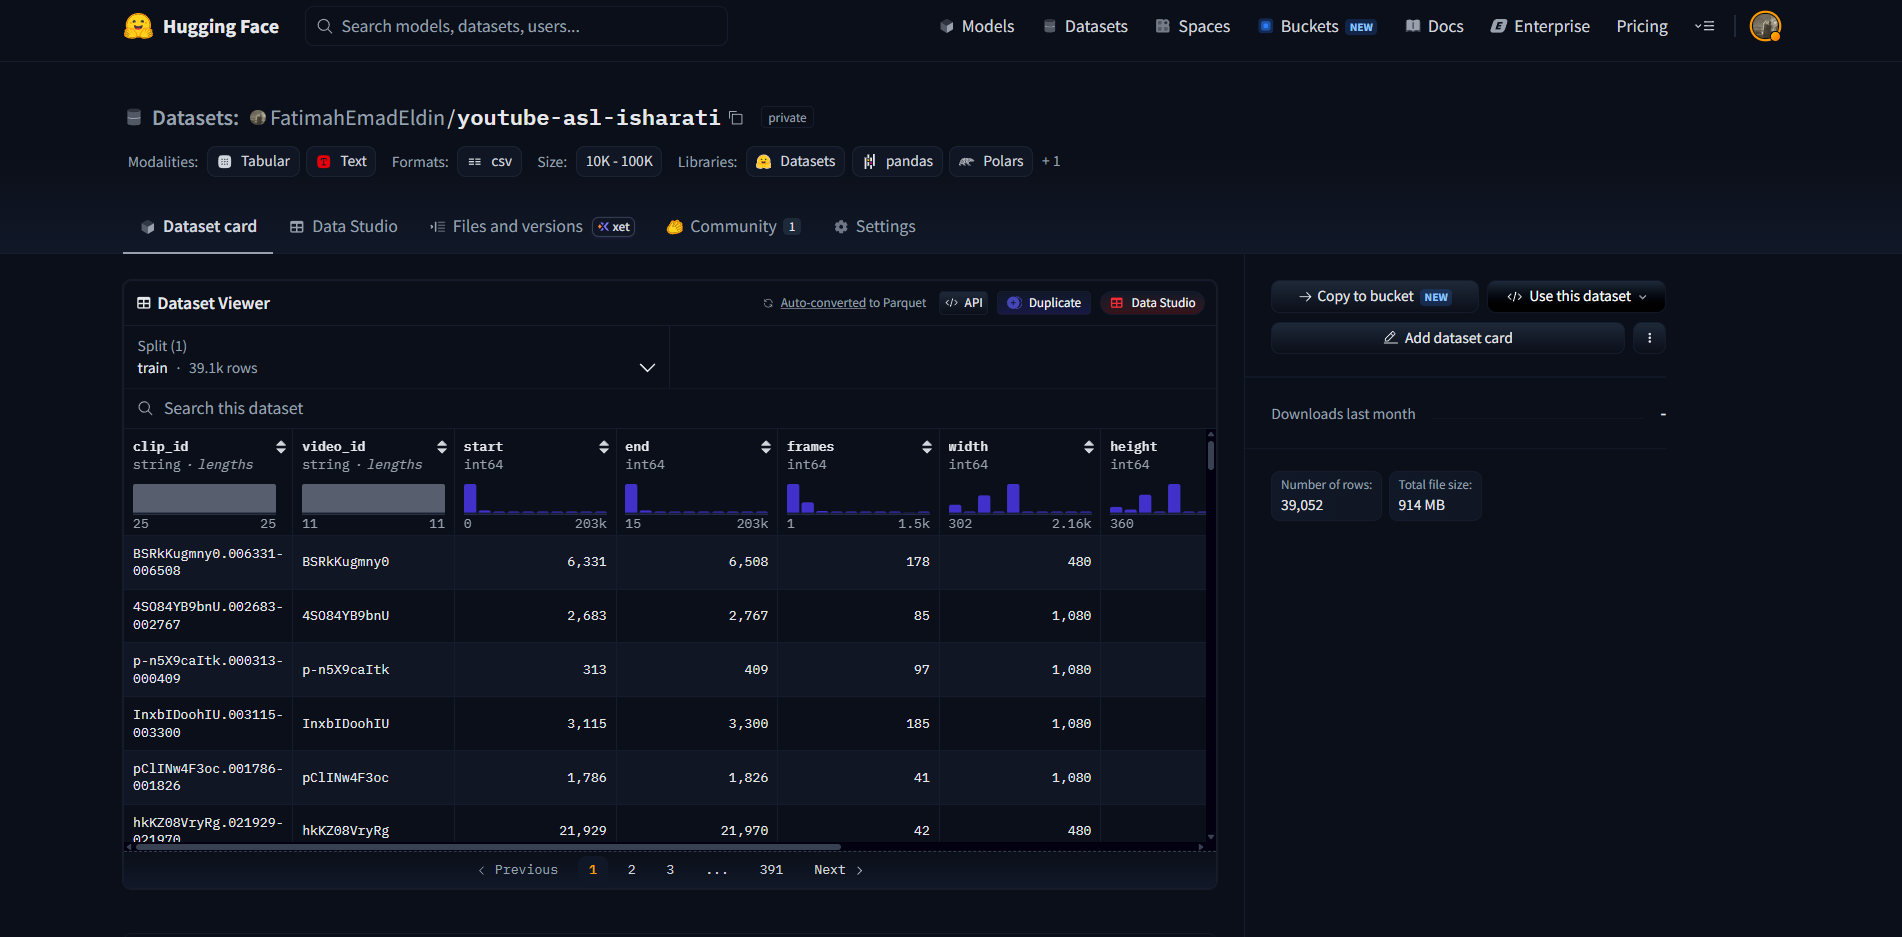
\includegraphics[width=\textwidth]{figures/hf_dataset.png}
\caption{The converted YouTube-ASL dataset on Hugging Face (first part: 39,052 clips, one manifest row per clip).}
\label{fig:hf}
\end{figure}

The first part holds 39,052 clips from 7,818 videos; 99.7\% are matched to their English sentence. Clips last a median
of 107 frames (about 3.6\,s; 5th--95th percentile 36--300), and 96\% have a hand detected in at least half of their
frames (Figure~\ref{fig:ytstats}); recordings range from 1080p webcams to 480p phones. These clips are used to train the
weakly supervised sign spotter of Chapter~\ref{sec:results}; 407 of the 500 most frequent uncovered Qur'an and hadith
words occur in the captions of this part alone.

\begin{figure}[ht]
\centering
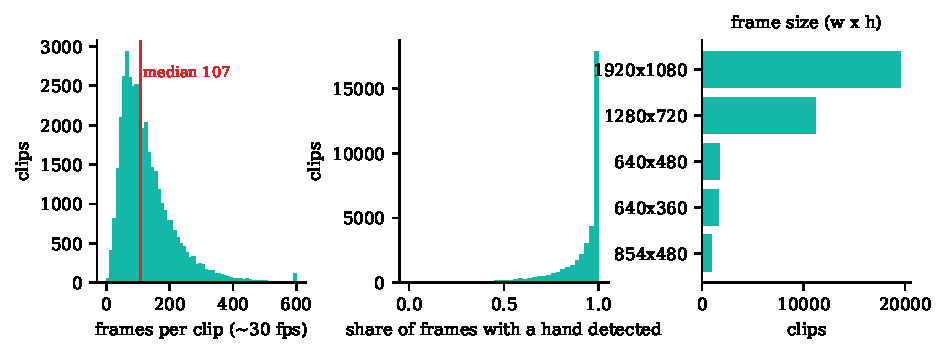
\includegraphics[width=\textwidth]{figures/youtube_asl_stats.pdf}
\caption{The first converted part of YouTube-ASL: clip length (red: median), share of frames with a hand detected, and
the most common frame sizes.}
\label{fig:ytstats}
\end{figure}
